% ============================================================================
%  Erdos Problem 915 -- seminarie deck (rebuild, Sept 2026)
%  Outline dictated by Louis: translation, E+V=G, the lambda cascade, the
%  kappa cascade, the red/blue pill model choices, then the program half
%  (modelling, max flow, transformations, efficiency, solving vs searching).
%
%  Self-contained, exactly like main.tex in this directory: the colours, the
%  graph vocabulary and the theme are copied from ../../preamble.tex so the
%  file builds on its own.
%
%  Build:  cd slides/seminarie && latexmk -pdf seminarie.tex
% ============================================================================
\documentclass[aspectratio=1610,11pt]{beamer}

\usepackage[T1]{fontenc}
\usepackage[utf8]{inputenc}
\usepackage{helvet}
\renewcommand{\familydefault}{\sfdefault}
\usepackage{amsmath,amssymb}
\usepackage{booktabs}
\usepackage{array}
\usepackage{multirow}
\usepackage{tabularx}
\usepackage{graphicx}
\usepackage{adjustbox}
\usepackage{tikz}
\usetikzlibrary{calc,arrows.meta,positioning,backgrounds,fit,shadows,decorations.markings}

\graphicspath{{../../figures/}{../../}}

% ============================================================================
%  COLOURS  (KU Leuven palette + the thesis's semantic graph colours)
% ============================================================================
\definecolor{KULblauw1}{RGB}{29,141,176}
\definecolor{KULblauw3a}{RGB}{82,189,236}
\definecolor{KULblauw3b}{RGB}{30,110,135}
\definecolor{vertexred}{RGB}{200,80,80}
\definecolor{vertexpurple}{RGB}{140,80,160}
\definecolor{vertexgreen}{RGB}{60,160,80}
\definecolor{vertexorange}{RGB}{220,140,40}

\definecolor{metroA}{RGB}{200,80,80}
\definecolor{metroB}{RGB}{29,141,176}
\definecolor{metroC}{RGB}{60,160,80}
\definecolor{metroD}{RGB}{220,140,40}
\definecolor{metroE}{RGB}{140,80,160}
\definecolor{metroF}{RGB}{120,120,120}

\definecolor{roleModel}{RGB}{82,189,236}
\definecolor{roleMeasure}{RGB}{29,141,176}
\definecolor{roleProve}{RGB}{60,160,80}
\definecolor{roleDiscover}{RGB}{220,140,40}

% the two pills of the model choice
\definecolor{pillRed}{RGB}{198,52,52}
\definecolor{pillBlue}{RGB}{40,110,190}

\colorlet{regimeProved}{KULblauw1}
\colorlet{regimeConjectured}{vertexred}
\colorlet{regimeOpen}{vertexorange}
\colorlet{regimePartial}{vertexpurple}

\definecolor{vtProved}{HTML}{1D8DB0}
\definecolor{vtConjectured}{HTML}{E05050}
\definecolor{vtOpen}{HTML}{E6B800}
\definecolor{vtExact}{HTML}{3CA050}
\definecolor{vtSearch}{HTML}{9B5DE5}

% ============================================================================
%  THE CANONICAL THESIS GRAPH VOCABULARY  (copied from preamble.tex)
% ============================================================================
\tikzset{
  gvertex/.style={circle, draw=KULblauw1, fill=KULblauw1!15, line width=1pt,
                  minimum size=6mm, inner sep=0pt, font=\small,
                  drop shadow={shadow xshift=0.4pt, shadow yshift=-0.5pt,
                               fill=black, opacity=0.18}},
  gline/.style ={line width=1.3pt, KULblauw1!75, line cap=round},
  gfaint/.style={line width=0.9pt, KULblauw1!40, line cap=round},
  gvhub/.style ={gvertex, draw=vertexorange, fill=vertexorange!18},
  gvsink/.style={gvertex, draw=vertexred,    fill=vertexred!15},
  gvcut/.style ={gvertex, draw=vertexpurple, fill=vertexpurple!20},
  gvnew/.style ={gvertex, draw=vertexorange, fill=vertexorange!22},
  gmulti/.style={gline},
  gdir/.style     ={-{Stealth[length=2.2mm]}, line width=1.1pt, KULblauw1!75, line cap=round},
  gdirfaint/.style={-{Stealth[length=1.8mm]}, line width=0.8pt, KULblauw1!40, line cap=round},
  gcut/.style     ={-{Stealth[length=2.2mm]}, line width=1.2pt, densely dashed, vertexred},
  gcutedge/.style ={line width=1.2pt, densely dashed, vertexred},
  grA/.style={line width=2.6pt, vertexorange,        line cap=round},
  grB/.style={line width=2.6pt, vertexgreen!70!black, line cap=round},
  grC/.style={line width=2.6pt, vertexpurple,         line cap=round},
  grAd/.style={grA, -{Stealth[length=2.8mm]}},
  grBd/.style={grB, -{Stealth[length=2.8mm]}},
  grCd/.style={grC, -{Stealth[length=2.8mm]}},
  gcurve/.style ={bend left=14},
  gcurveR/.style={bend right=14},
  vertex/.style={gvertex},
  smallvertex/.style={gvertex, minimum size=16pt, font=\scriptsize},
  edge/.style={gline},
  arc/.style={gdir},
  metro/.style={line width=3.4pt, line cap=round, line join=round, rounded corners=4pt},
  metrostop/.style={circle, draw=black!72, fill=white, line width=1pt,
                     minimum size=6mm, inner sep=0pt, font=\scriptsize\bfseries},
  hnode/.style={rectangle, draw=KULblauw3b, fill=white, minimum size=13pt,
                inner sep=1pt, line width=1pt, font=\scriptsize\bfseries},
  vtroot/.style={rectangle, rounded corners=3pt, draw=KULblauw3b, very thick,
                 minimum width=26mm, minimum height=9mm, font=\sffamily\small\bfseries},
  vtmodel/.style={rectangle, rounded corners=3pt, draw=KULblauw3b, thick,
                  minimum width=20mm, minimum height=8mm, font=\sffamily\small},
  vtdir/.style={rectangle, rounded corners=2.5pt, draw=KULblauw3b!70,
                minimum width=19mm, minimum height=7mm, font=\scriptsize},
  vtleaf/.style={rectangle, rounded corners=2pt, draw=KULblauw3b!70,
                 minimum width=12mm, minimum height=6.5mm, font=\scriptsize},
  vtedge/.style={KULblauw3b!55, line width=0.9pt},
}

% ---- styles this deck adds: the definition cascade of frames 3 and 4 -------
% A formula is split across several nodes glued at their baselines, so the
% token being defined is its own node an arrow can leave from.
\tikzset{
  form/.style={inner sep=1pt, outer sep=0pt, font=\large},
  tok/.style={inner xsep=4pt, inner ysep=3pt, outer sep=0pt, font=\large,
              rounded corners=2.5pt, fill=KULblauw3a!22, draw=KULblauw1!55,
              line width=0.8pt},
  tokv/.style={tok, fill=vertexpurple!18, draw=vertexpurple!65},
  casc/.style={-{Stealth[length=2.6mm]}, line width=1.1pt, KULblauw1!70},
  cascv/.style={casc, draw=vertexpurple!70},
  saying/.style={font=\footnotesize\itshape, text=black!55},
}

% ============================================================================
%  NOTATION SHORTHANDS  (copied from preamble.tex)
% ============================================================================
\newcommand*{\floor}[1]{\left\lfloor #1 \right\rfloor}
\newcommand*{\floorfrac}[2]{\floor{\frac{#1}{#2}}}
\newcommand{\lec}{\lambda}
\newcommand{\kap}{\kappa}
\newcommand{\lmax}{\lambda^{\max}}
\newcommand{\kmax}{\kappa^{\max}}
\newcommand{\dir}{\mathrm{dir}}
\newcommand{\HH}{\mathcal{H}}
\newcommand{\Erdos}{Erd\H{o}s}
\newtheorem{proposition}{Proposition}
% carried over from ../../preamble.tex: marks a result whose proof here was
% written by an AI model and not checked line by line by the author.
\newcommand{\aimedal}{\,[AI]}

% ============================================================================
%  THEME
% ============================================================================
\setbeamertemplate{navigation symbols}{}
\usefonttheme{professionalfonts}
\setbeamercolor{structure}{fg=KULblauw1}
\setbeamercolor{frametitle}{fg=KULblauw3b}
\setbeamercolor{title}{fg=KULblauw3b}
\setbeamercolor{normal text}{fg=black!88}
\setbeamercolor{itemize item}{fg=KULblauw1}
\setbeamerfont{frametitle}{series=\bfseries,size=\large}
\setbeamerfont{title}{series=\bfseries}
\setbeamertemplate{itemize item}{\small\raise0.5pt\hbox{\textbullet}}

\setbeamertemplate{frametitle}{%
  \vskip4pt%
  \begin{beamercolorbox}[wd=\paperwidth,leftskip=0.9cm,rightskip=0.9cm]{frametitle}%
    \usebeamerfont{frametitle}\insertframetitle%
  \end{beamercolorbox}%
  \vskip2pt%
  \hspace*{0.9cm}{\color{KULblauw3a}\rule{0.82\paperwidth}{1.1pt}}%
  \vskip1pt%
}

\setbeamertemplate{footline}{%
  \hbox{%
    \begin{beamercolorbox}[wd=0.72\paperwidth,ht=2.4ex,dp=1.2ex,leftskip=0.9cm]{}%
      {\scriptsize\color{black!45}\Erdos{} Problem 915}%
    \end{beamercolorbox}%
    \begin{beamercolorbox}[wd=0.28\paperwidth,ht=2.4ex,dp=1.2ex,rightskip=0.9cm]{}%
      \hfill{\scriptsize\color{black!45}\insertframenumber\,/\,\inserttotalframenumber}%
    \end{beamercolorbox}%
  }%
}
\setbeamersize{text margin left=0.9cm,text margin right=0.9cm}

% ============================================================================
%  FRAME BUILDERS
% ============================================================================
\newcommand{\figframe}[3]{%
  \begin{frame}{#1}
    \vfill
    \begin{center}
    \includegraphics[width=\textwidth,height=0.66\textheight,keepaspectratio]{#2}
    \end{center}
    \vspace{3pt}
    \noindent{\footnotesize\color{black!60} #3}\par
    \vfill
  \end{frame}%
}
\newcommand{\figframetall}[3]{%
  \begin{frame}{#1}
    \vspace{-2pt}
    \begin{center}
    \includegraphics[width=\textwidth,height=0.66\textheight,keepaspectratio]{#2}
    \end{center}
    \vspace{1pt}
    \noindent{\tiny\color{black!60} #3}\par
  \end{frame}%
}
\newcommand{\tikzframescaled}[4]{%
  \begin{frame}{#1}
    \vfill
    \begin{center}
    \adjustbox{max totalheight=0.64\textheight}{\resizebox{#4\textwidth}{!}{#2}}
    \end{center}
    \vspace{8pt}
    \noindent{\footnotesize\color{black!60} #3}\par
    \vfill
  \end{frame}%
}
\newcommand{\tikzframe}[3]{\tikzframescaled{#1}{#2}{#3}{1.0}}

% --- a capsule, for the model-choice frames --------------------------------
% #1 colour, #2 rotation in degrees, #3 scale
\newcommand{\pillshape}[3]{%
  \begin{scope}[rotate=#2, scale=#3]
    \begin{scope}
      \clip[rounded corners=4.5mm] (-1.55,-0.45) rectangle (1.55,0.45);
      \fill[#1!88!black] (-1.55,-0.45) rectangle (1.55,0.45);
      \fill[#1!42!white] (-1.55,-0.45) rectangle (0,0.45);
      \fill[white, opacity=0.28] (-1.42,0.10) rectangle (1.30,0.29);
      \fill[black, opacity=0.10] (-0.03,-0.45) rectangle (0.03,0.45);
    \end{scope}
    \draw[black!30, line width=0.7pt, rounded corners=4.5mm]
      (-1.55,-0.45) rectangle (1.55,0.45);
  \end{scope}}

% a small pill used as a bullet-sized icon
\newcommand{\pillicon}[1]{%
  \tikz[baseline=-0.6ex]{\pillshape{#1}{-18}{0.34}}}

% one row of the transformation frame: a caption column and a picture column
% clamped independently, so neither can ever run into the other
\newcommand{\transrow}[3]{%
  \noindent
  \parbox[c]{0.235\textwidth}{\raggedright
    {\footnotesize\color{KULblauw3b}\bfseries #1}\\[2pt]
    {\scriptsize\color{black!55} #2}}%
  \hfill
  \parbox[c]{0.735\textwidth}{\centering
    \adjustbox{max width=0.72\linewidth, max totalheight=0.30\textheight}{#3}}\par}

\title{Maximising Edge Density Subject to Connectivity Constraints}
\author{Louis Vandenbruwaene}
\date{Academic Year 2026--2027}

\begin{document}

% ============================================================================
%  TITLE
% ============================================================================
\begin{frame}[plain]
\vspace{1.9cm}
\hspace*{0.5cm}\begin{minipage}{0.9\textwidth}
  {\color{black!40}\large EXTREMAL GRAPH THEORY}\\[10pt]
  {\color{KULblauw3b}\fontsize{32}{36}\selectfont\bfseries \Erdos{} Problem 915}\\[8pt]
  {\color{KULblauw1}\Large Maximising Edge Density Subject to Connectivity Constraints}

  \vspace{1.4cm}
  {\large\bfseries Louis Vandenbruwaene}\\[3pt]
  {\small\color{black!70}Supervisor: Prof.\ Stijn Cambie \qquad Promotor: Prof.\ Jan Goedgebeur}\\[2pt]
  {\small\color{black!70}KU Leuven, Master of Mathematics}
\end{minipage}
\begin{tikzpicture}[remember picture,overlay]
  \node[anchor=south east] at ($(current page.south east)+(-0.8,0.5)$)
    {
\includegraphics[height=1.0cm]{LogoKULeuven.png}};
\end{tikzpicture}
\end{frame}

% ============================================================================
%  1.  THE TITLE, TRANSLATED
% ============================================================================
\begin{frame}{The title, in plain words}
\vfill
\begin{center}
\adjustbox{max totalheight=0.70\textheight}{\resizebox{0.94\textwidth}{!}{%
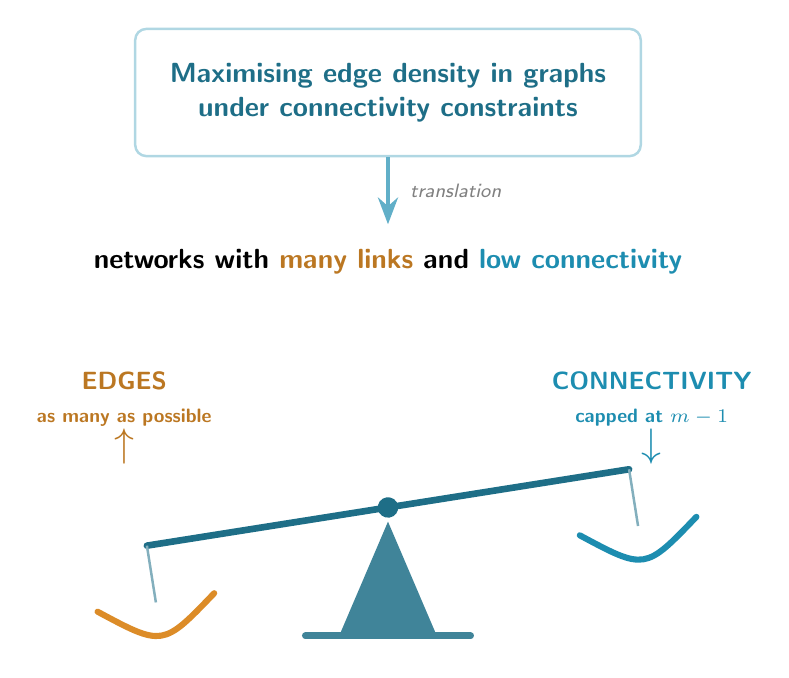
\begin{tikzpicture}
  % --- the formal title ---------------------------------------------------
  \node[font=\bfseries, text=KULblauw3b, align=center] (formal) at (0,3.9)
    {Maximising edge density in graphs\\under connectivity constraints};
  \node[draw=KULblauw1!35, rounded corners=4pt, line width=0.9pt,
        fit={(formal)}, inner sep=9pt] (fbox) {};

  % --- the translation arrow ----------------------------------------------
  \draw[-{Stealth[length=3.4mm]}, line width=1.4pt, KULblauw1!70]
    (fbox.south) -- ++(0,-0.85)
    node[midway, right=4pt, font=\scriptsize\itshape, text=black!50] {translation};

  % --- the plain sentence -------------------------------------------------
  \node[font=\bfseries, align=center] (plain) at (0,1.75)
    {networks with {\color{vertexorange!85!black}many links}
     and {\color{KULblauw1}low connectivity}};

  % --- the balance ---------------------------------------------------------
  \begin{scope}[shift={(0,-1.55)}]
    % stand
    \fill[KULblauw3b!85] (0,0) -- (-0.62,-1.45) -- (0.62,-1.45) -- cycle;
    \draw[line width=2.4pt, KULblauw3b!85, line cap=round] (-1.05,-1.45) -- (1.05,-1.45);
    % the beam tips to the left: the edge side is the heavy one
    \begin{scope}[rotate around={9:(0,0.18)}]
      \draw[line width=2.4pt, KULblauw3b, line cap=round] (-3.1,0.18) -- (3.1,0.18);
      \fill[KULblauw3b] (0,0.18) circle (0.13);
      % left pan: edges
      \draw[line width=0.9pt, KULblauw3b!55] (-3.1,0.18) -- (-3.1,-0.55);
      \draw[line width=2.2pt, vertexorange, line cap=round]
        (-3.85,-0.55) .. controls (-3.1,-1.12) .. (-2.35,-0.55);
      % right pan: connectivity
      \draw[line width=0.9pt, KULblauw3b!55] (3.1,0.18) -- (3.1,-0.55);
      \draw[line width=2.2pt, KULblauw1, line cap=round]
        (2.35,-0.55) .. controls (3.1,-1.12) .. (3.85,-0.55);
    \end{scope}
    % pan labels, upright and clear of the beam
    \node[font=\small\bfseries, text=vertexorange!85!black, align=center]
      at (-3.35,1.55) {EDGES\\[1pt]{\scriptsize as many as possible}};
    \node[font=\small\bfseries, text=KULblauw1, align=center]
      at (3.35,1.55) {CONNECTIVITY\\[1pt]{\scriptsize capped at $m-1$}};
    \node[font=\Large\bfseries, text=vertexorange!85!black] at (-3.35,0.95) {$\uparrow$};
    \node[font=\Large\bfseries, text=KULblauw1]             at (3.35,0.95) {$\downarrow$};
  \end{scope}
\end{tikzpicture}}}
\end{center}
\vspace{4pt}
\noindent{\footnotesize\color{black!60}
Push the edge count up while holding every pair of vertices weakly joined. The
whole thesis is that one trade-off, asked over and over in different models.}\par
\vfill
\end{frame}

% ============================================================================
%  2.  E + V = G
% ============================================================================
\begin{frame}{A graph is edges and vertices}
\vfill
\begin{center}
\adjustbox{max totalheight=0.68\textheight}{\resizebox{0.96\textwidth}{!}{%
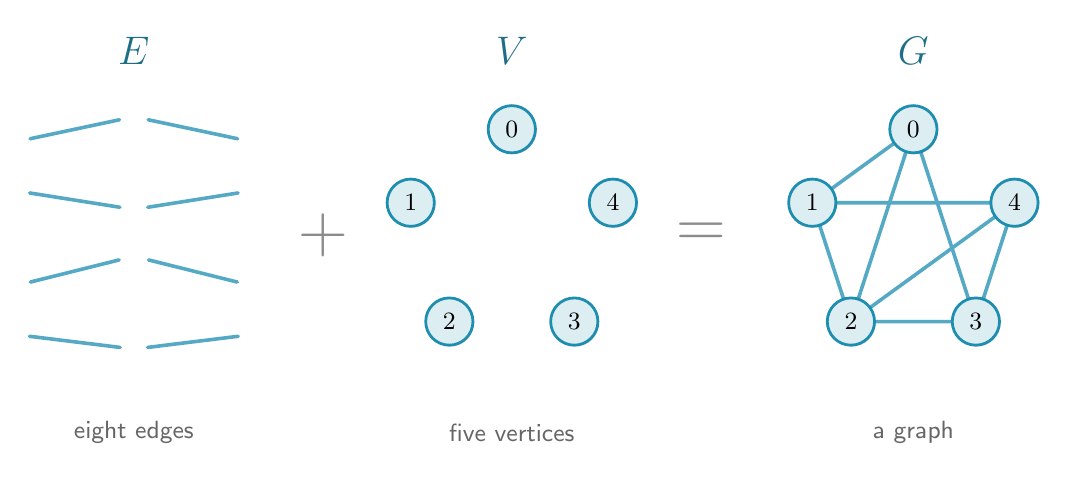
\begin{tikzpicture}
  % ---- E: eight loose edges, no endpoints ---------------------------------
  \begin{scope}[shift={(0,0)}]
    \foreach \i/\x/\y/\a in {1/-0.75/1.35/12, 2/0.75/1.35/-12,
                             3/-0.75/0.45/-9, 4/0.75/0.45/9,
                             5/-0.75/-0.45/14, 6/0.75/-0.45/-14,
                             7/-0.75/-1.35/-7, 8/0.75/-1.35/7} {
      \draw[gline, rotate around={\a:(\x,\y)}] (\x-0.58,\y) -- (\x+0.58,\y);
    }
    \node[font=\bfseries\Large, text=KULblauw3b] at (0,2.35) {$E$};
    \node[font=\small, text=black!60] at (0,-2.5) {eight edges};
  \end{scope}

  \node[font=\Huge, text=black!45] at (2.4,0) {$+$};

  % ---- V: five loose vertices ---------------------------------------------
  \begin{scope}[shift={(4.8,0)}]
    \foreach \i in {0,...,4} {
      \pgfmathsetmacro{\ang}{90 + 72*\i}
      \node[gvertex] at (\ang:1.35) {$\i$};
    }
    \node[font=\bfseries\Large, text=KULblauw3b] at (0,2.35) {$V$};
    \node[font=\small, text=black!60] at (0,-2.5) {five vertices};
  \end{scope}

  \node[font=\Huge, text=black!45] at (7.2,0) {$=$};

  % ---- G: the two put together --------------------------------------------
  \begin{scope}[shift={(9.9,0)}]
    \foreach \i in {0,...,4} {
      \pgfmathsetmacro{\ang}{90 + 72*\i}
      \coordinate (v\i) at (\ang:1.35);
    }
    \draw[gline] (v0)--(v1) (v0)--(v2) (v0)--(v3)
                 (v1)--(v2) (v1)--(v4)
                 (v2)--(v3) (v2)--(v4)
                 (v3)--(v4);
    \foreach \i in {0,...,4} {
      \pgfmathsetmacro{\ang}{90 + 72*\i}
      \node[gvertex] at (\ang:1.35) {$\i$};
    }
    \node[font=\bfseries\Large, text=KULblauw3b] at (0,2.35) {$G$};
    \node[font=\small, text=black!60] at (0,-2.5) {a graph};
  \end{scope}
\end{tikzpicture}}}
\end{center}
\vspace{6pt}
\noindent{\footnotesize\color{black!60}
An edge joins a pair of vertices, and $|E(G)|$ is the number being maximised.
The picture is $K_5-\{04,13\}$, the running example: five vertices, eight
edges.}\par
\vfill
\end{frame}

% ============================================================================
%  3.  ERDOS 915, UNFOLDED  (edge version)
% ============================================================================
\begin{frame}{\Erdos{} Problem 915}
\vspace{-2pt}
\begin{center}
\adjustbox{max totalheight=0.74\textheight}{\resizebox{0.99\textwidth}{!}{%
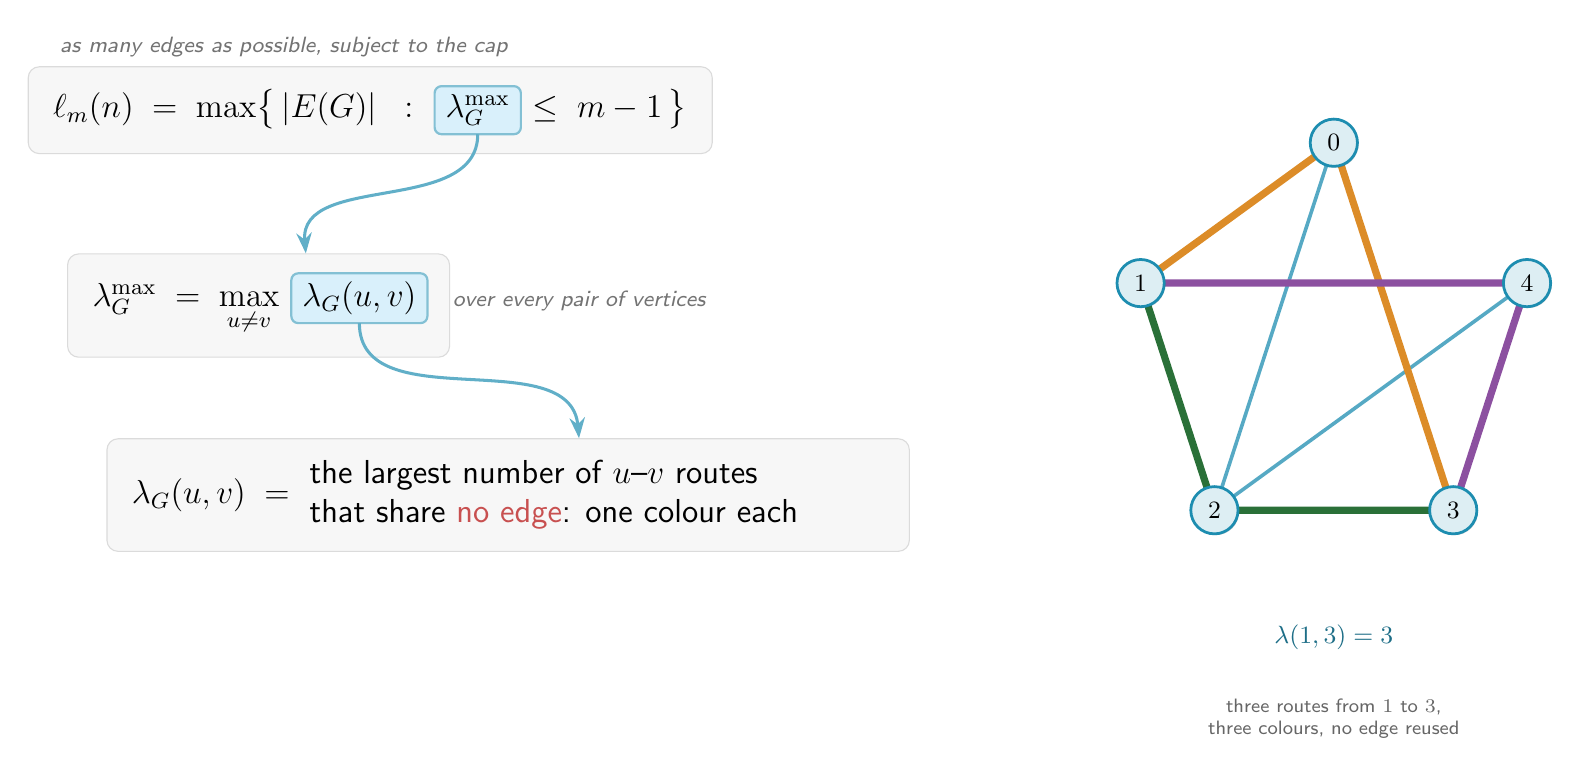
\begin{tikzpicture}[
   cbox/.style={draw=black!14, fill=black!3, rounded corners=4pt,
                inner xsep=8pt, inner ysep=7pt}]

  % ---- the problem ---------------------------------------------------------
  \node[form, anchor=base west] (a1) at (-6.4,3.5)
    {$\ell_m(n)\;=\;\max\bigl\{\,|E(G)|\;\;:\;\;$};
  \node[tok, anchor=base west] (a2) at (a1.base east) {$\lmax_G$};
  \node[form, anchor=base west] (a3) at (a2.base east) {$\;\le\;m-1\,\bigr\}$};
  \node[saying, anchor=south west] at (-6.4,4.15)
    {as many edges as possible, subject to the cap};

  % ---- the graph-wide maximum ---------------------------------------------
  \node[form, anchor=base west] (b1) at (-5.9,1.1)
    {$\lmax_G\;=\;\max\limits_{u\neq v}\;$};
  \node[tok, anchor=base west] (b2) at (b1.base east) {$\lec_G(u,v)$};
  \node[saying, anchor=base west] at (b2.base east)
    {\ \ over every pair of vertices};

  % ---- the local quantity --------------------------------------------------
  \node[form, anchor=base west, align=left] (c1) at (-5.4,-1.4)
    {$\lec_G(u,v)\;=\;$
     \begin{minipage}{7.3cm}
       the largest number of $u$--$v$ routes\\
       that share {\color{vertexred}no edge}: one colour each
     \end{minipage}};

  \begin{scope}[on background layer]
    \node[cbox, fit=(a1)(a2)(a3)] (boxA) {};
    \node[cbox, fit=(b1)(b2)]     (boxB) {};
    \node[cbox, fit=(c1)]         (boxC) {};
  \end{scope}

  \draw[casc] (a2.south) to[out=-90,in=95] ($(boxB.north)+(0.6,0)$);
  \draw[casc] (b2.south) to[out=-90,in=95] ($(boxC.north)+(0.9,0)$);

  % ---- the picture: Menger's routes, without the cut -----------------------
  \begin{scope}[shift={(9.9,0.6)}, scale=1.72]
    \foreach \i in {0,...,4} {
      \pgfmathsetmacro{\ang}{90 + 72*\i}
      \coordinate (v\i) at (\ang:1.5);
    }
    \draw[gline] (v0)--(v1) (v0)--(v2) (v0)--(v3)
                 (v1)--(v2) (v1)--(v4)
                 (v2)--(v3) (v2)--(v4)
                 (v3)--(v4);
    \draw[grA] (v1)--(v0)--(v3);
    \draw[grB] (v1)--(v2)--(v3);
    \draw[grC] (v1)--(v4)--(v3);
    \foreach \i in {0,...,4} {
      \pgfmathsetmacro{\ang}{90 + 72*\i}
      \node[gvertex] at (\ang:1.5) {$\i$};
    }
    \node[font=\small\bfseries, text=KULblauw3b] at (0,-2.15) {$\lec(1,3)=3$};
    \node[font=\scriptsize, text=black!60, align=center] at (0,-2.75)
      {three routes from $1$ to $3$,\\three colours, no edge reused};
  \end{scope}
\end{tikzpicture}}}
\end{center}
\vspace{2pt}
\noindent{\footnotesize\color{black!60}
Menger's theorem gives the same number a second face: $\lec_G(u,v)$ is also the
fewest edges whose removal cuts every $u$--$v$ route. That is the face the
program will measure.}\par
\end{frame}

% ============================================================================
%  4.  THE SAME QUESTION UNDER VERTEX SEPARATION
% ============================================================================
\begin{frame}{The same question, vertex by vertex}
\vspace{-2pt}
\begin{center}
\adjustbox{max totalheight=0.74\textheight}{\resizebox{0.99\textwidth}{!}{%
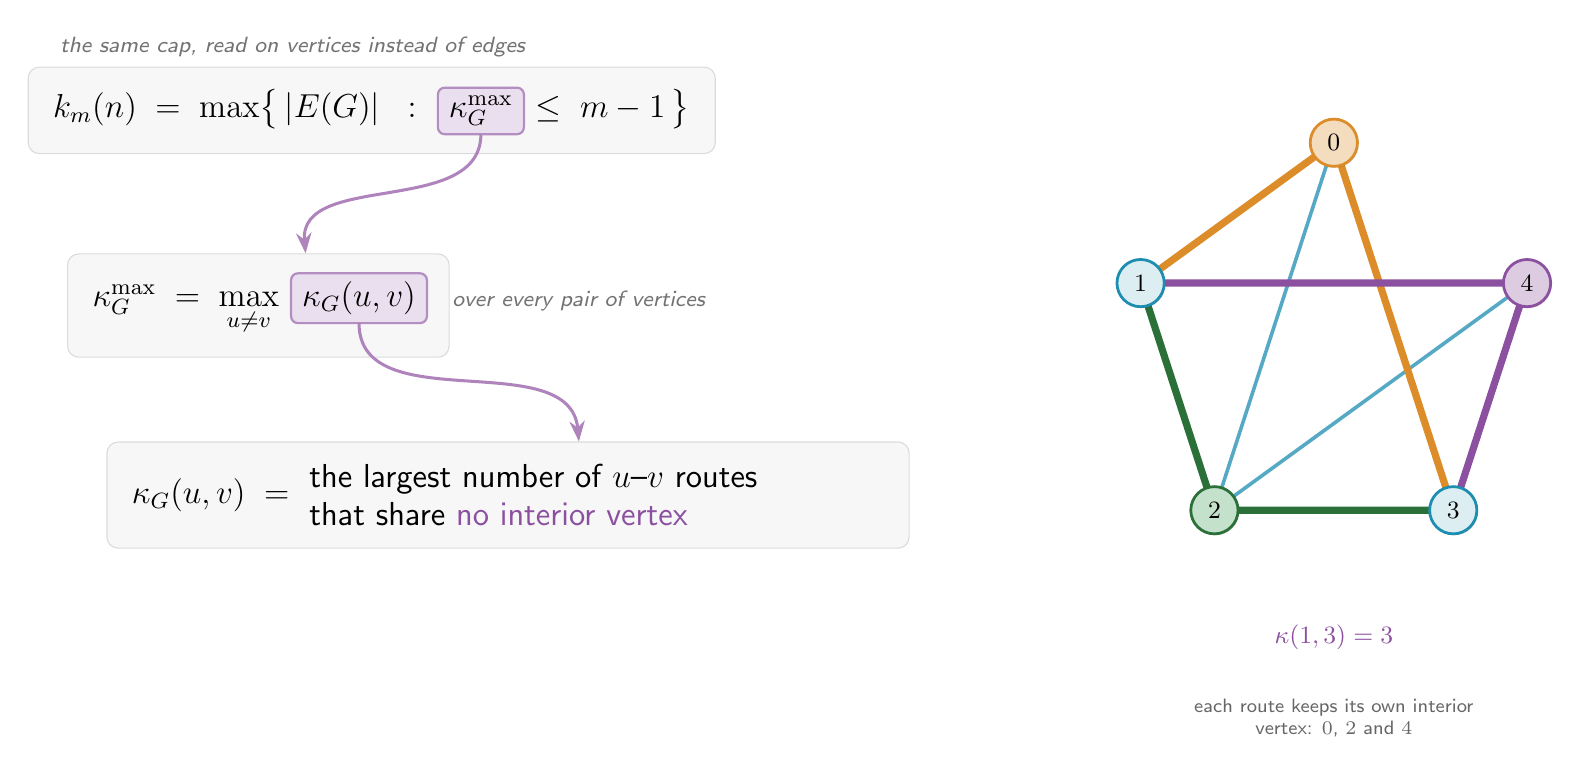
\begin{tikzpicture}[
   cbox/.style={draw=black!14, fill=black!3, rounded corners=4pt,
                inner xsep=8pt, inner ysep=7pt}]

  \node[form, anchor=base west] (a1) at (-6.4,3.5)
    {$k_m(n)\;=\;\max\bigl\{\,|E(G)|\;\;:\;\;$};
  \node[tokv, anchor=base west] (a2) at (a1.base east) {$\kmax_G$};
  \node[form, anchor=base west] (a3) at (a2.base east) {$\;\le\;m-1\,\bigr\}$};
  \node[saying, anchor=south west] at (-6.4,4.15)
    {the same cap, read on vertices instead of edges};

  \node[form, anchor=base west] (b1) at (-5.9,1.1)
    {$\kmax_G\;=\;\max\limits_{u\neq v}\;$};
  \node[tokv, anchor=base west] (b2) at (b1.base east) {$\kap_G(u,v)$};
  \node[saying, anchor=base west] at (b2.base east)
    {\ \ over every pair of vertices};

  \node[form, anchor=base west, align=left] (c1) at (-5.4,-1.4)
    {$\kap_G(u,v)\;=\;$
     \begin{minipage}{7.3cm}
       the largest number of $u$--$v$ routes\\
       that share {\color{vertexpurple}no interior vertex}
     \end{minipage}};

  \begin{scope}[on background layer]
    \node[cbox, fit=(a1)(a2)(a3)] (boxA) {};
    \node[cbox, fit=(b1)(b2)]     (boxB) {};
    \node[cbox, fit=(c1)]         (boxC) {};
  \end{scope}

  \draw[cascv] (a2.south) to[out=-90,in=95] ($(boxB.north)+(0.6,0)$);
  \draw[cascv] (b2.south) to[out=-90,in=95] ($(boxC.north)+(0.9,0)$);

  % ---- the picture: now the interior VERTICES carry the colours ------------
  \begin{scope}[shift={(9.9,0.6)}, scale=1.72]
    \foreach \i in {0,...,4} {
      \pgfmathsetmacro{\ang}{90 + 72*\i}
      \coordinate (v\i) at (\ang:1.5);
    }
    \draw[gline] (v0)--(v1) (v0)--(v2) (v0)--(v3)
                 (v1)--(v2) (v1)--(v4)
                 (v2)--(v3) (v2)--(v4)
                 (v3)--(v4);
    \draw[grA] (v1)--(v0)--(v3);
    \draw[grB] (v1)--(v2)--(v3);
    \draw[grC] (v1)--(v4)--(v3);
    % endpoints stay house blue, the three interior vertices take a colour each
    \node[gvertex] at (v1) {$1$};
    \node[gvertex] at (v3) {$3$};
    \node[gvertex, draw=vertexorange,  fill=vertexorange!30]  at (v0) {$0$};
    \node[gvertex, draw=vertexgreen!70!black, fill=vertexgreen!30] at (v2) {$2$};
    \node[gvertex, draw=vertexpurple,  fill=vertexpurple!30]  at (v4) {$4$};
    \node[font=\small\bfseries, text=vertexpurple] at (0,-2.15) {$\kap(1,3)=3$};
    \node[font=\scriptsize, text=black!60, align=center] at (0,-2.75)
      {each route keeps its own interior\\vertex: $0$, $2$ and $4$};
  \end{scope}
\end{tikzpicture}}}
\end{center}
\vspace{2pt}
\noindent{\footnotesize\color{black!60}
Whitney's inequality $\kap_G(u,v)\le\lec_G(u,v)$: avoiding shared vertices is at
least as demanding as avoiding shared edges. Here the two agree, but they need
not.}\par
\end{frame}

% ============================================================================
%  4b.  WHERE THE TWO PART COMPANY
% ============================================================================
\tikzframescaled{Where the two part company}{%
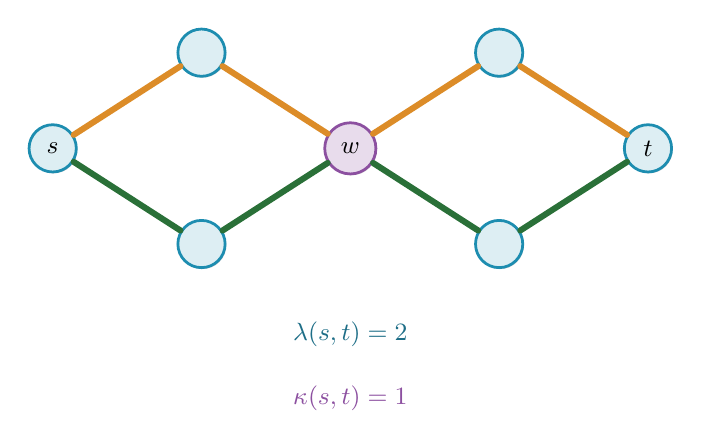
\begin{tikzpicture}[scale=1.35,
    pA/.style={grA, line width=2.2pt},
    pB/.style={grB, line width=2.2pt}]
  \node[gvertex]  (s) at (0,0)      {$s$};
  \node[gvertex]  (a) at (1.4,0.9)  {};
  \node[gvertex]  (c) at (1.4,-0.9) {};
  \node[gvcut, minimum size=6.5mm] (w) at (2.8,0) {$w$};
  \node[gvertex]  (b) at (4.2,0.9)  {};
  \node[gvertex]  (d) at (4.2,-0.9) {};
  \node[gvertex]  (t) at (5.6,0)    {$t$};
  \draw[pA] (s)--(a)--(w)--(b)--(t);
  \draw[pB] (s)--(c)--(w)--(d)--(t);
  \node[font=\small, text=KULblauw3b]  at (2.8,-1.75) {$\lec(s,t)=2$};
  \node[font=\small, text=vertexpurple] at (2.8,-2.35) {$\kap(s,t)=1$};
\end{tikzpicture}}{%
Two routes that share no edge are still forced through the single vertex $w$.
Every toggle in this thesis is chosen because it moves the answer, and this one
does.}{0.66}

% ============================================================================
%  5.  THE CHOICE: THREE TOGGLES
% ============================================================================
{
\setbeamercolor{background canvas}{bg=black!92}
\setbeamercolor{normal text}{fg=white}
\usebeamercolor[fg]{normal text}
\begin{frame}[plain]
\vspace{0.7cm}
\begin{center}
{\color{white!70}\large THREE CHOICES TO MAKE}\\[0.9cm]
\adjustbox{max totalheight=0.52\textheight}{\resizebox{0.80\textwidth}{!}{%
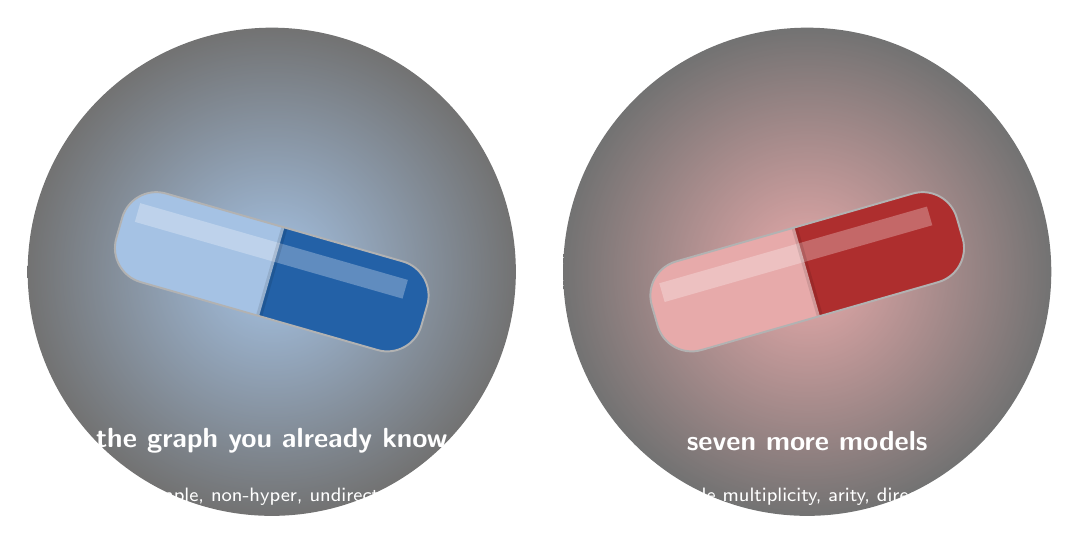
\begin{tikzpicture}
  \shade[inner color=pillBlue!70, outer color=black!92, opacity=0.60]
    (-3.4,0) circle (3.1);
  \shade[inner color=pillRed!70, outer color=black!92, opacity=0.60]
    (3.4,0) circle (3.1);
  \begin{scope}[shift={(-3.4,0)}]\pillshape{pillBlue}{-16}{1.30}\end{scope}
  \begin{scope}[shift={(3.4,0)}]\pillshape{pillRed}{16}{1.30}\end{scope}
  \node[font=\bfseries, text=white, align=center] at (-3.4,-2.15)
    {the graph you already know};
  \node[font=\bfseries, text=white, align=center] at (3.4,-2.15)
    {seven more models};
  \node[font=\scriptsize, text=white!60, align=center] at (-3.4,-2.85)
    {simple, non-hyper, undirected};
  \node[font=\scriptsize, text=white!60, align=center] at (3.4,-2.85)
    {toggle multiplicity, arity, direction};
\end{tikzpicture}}}
\\[0.9cm]
{\color{white!80}\normalsize
$2\ \text{multiplicity}\;\times\;2\ \text{arity}\;\times\;2\ \text{direction}\;=\;8$ models,
\ and each is asked twice, for $\lec$ and for $\kap$: \textbf{16 variants}.}
\end{center}
\end{frame}
}

% ---- choice 1: multiplicity ------------------------------------------------
\begin{frame}{Choice 1 of 3: multiplicity}
\vspace{2pt}
\begin{columns}[T,onlytextwidth]
\column{0.47\textwidth}
\centering
{\pillicon{pillBlue}}\ \ {\large\bfseries simple}\\[2pt]
{\scriptsize\color{black!60} at most one edge per pair}\\[12pt]
\adjustbox{max totalheight=0.355\textheight, max width=\linewidth}{%
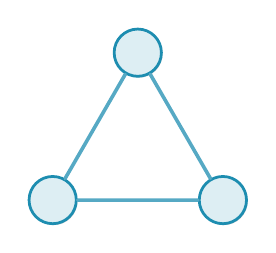
\begin{tikzpicture}[scale=1.6]
  \node[gvertex] (s1) at (90:0.78) {};
  \node[gvertex] (s2) at (210:0.78) {};
  \node[gvertex] (s3) at (330:0.78) {};
  \draw[gline] (s1)--(s2) (s2)--(s3) (s3)--(s1);
\end{tikzpicture}}\\[10pt]
{\footnotesize\color{black!60} $\mu(u,v)\in\{0,1\}$}

\column{0.06\textwidth}
\centering
\vspace{2.4cm}{\color{black!25}\large vs}

\column{0.47\textwidth}
\centering
{\pillicon{pillRed}}\ \ {\large\bfseries multigraph}\\[2pt]
{\scriptsize\color{black!60} parallel copies allowed}\\[12pt]
\adjustbox{max totalheight=0.355\textheight, max width=\linewidth}{%
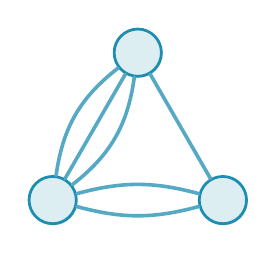
\begin{tikzpicture}[scale=1.6]
  \node[gvertex] (g1) at (90:0.78) {};
  \node[gvertex] (g2) at (210:0.78) {};
  \node[gvertex] (g3) at (330:0.78) {};
  \draw[gline] (g1) to[bend left=22] (g2);
  \draw[gline] (g1) -- (g2);
  \draw[gline] (g1) to[bend right=22] (g2);
  \draw[gline] (g2) to[bend left=15] (g3);
  \draw[gline] (g2) to[bend right=15] (g3);
  \draw[gline] (g3) -- (g1);
\end{tikzpicture}}\\[10pt]
{\footnotesize\color{black!60} $\mu(u,v)\in\{0,\ldots,m-1\}$}
\end{columns}
\vspace{10pt}
\noindent{\footnotesize\color{black!60}
A parallel copy is a route of its own, so the cap is spent on multiplicity
before it is spent on new neighbours. The extremal function is written
$L_m(n)$ rather than $\ell_m(n)$.}\par
\end{frame}

% ---- choice 2: arity -------------------------------------------------------
\begin{frame}{Choice 2 of 3: arity}
\vspace{2pt}
\begin{columns}[T,onlytextwidth]
\column{0.47\textwidth}
\centering
{\pillicon{pillBlue}}\ \ {\large\bfseries graph}\\[2pt]
{\scriptsize\color{black!60} every line serves two stops}\\[12pt]
\adjustbox{max totalheight=0.355\textheight, max width=\linewidth}{%
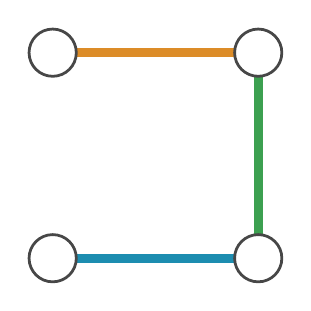
\begin{tikzpicture}[scale=1.45]
  \coordinate (A) at (-0.9,-0.9); \coordinate (B) at (0.9,-0.9);
  \coordinate (C) at (0.9, 0.9);  \coordinate (D) at (-0.9,0.9);
  \begin{scope}[on background layer]
    \draw[metro, metroB] (A) -- (B);
    \draw[metro, metroC] (B) -- (C);
    \draw[metro, metroD] (C) -- (D);
  \end{scope}
  \foreach \p in {A,B,C,D} {\node[metrostop] at (\p) {};}
\end{tikzpicture}}\\[10pt]
{\footnotesize\color{black!60} $r=2$}

\column{0.06\textwidth}
\centering
\vspace{2.4cm}{\color{black!25}\large vs}

\column{0.47\textwidth}
\centering
{\pillicon{pillRed}}\ \ {\large\bfseries hypergraph}\\[2pt]
{\scriptsize\color{black!60} a line serves three or more}\\[12pt]
\adjustbox{max totalheight=0.355\textheight, max width=\linewidth}{%
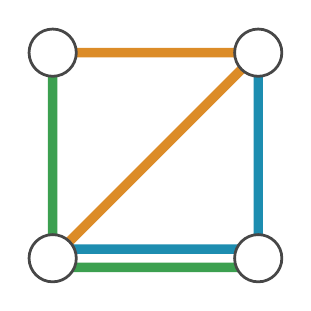
\begin{tikzpicture}[scale=1.45]
  \coordinate (A) at (-0.9,-0.9); \coordinate (B) at (0.9,-0.9);
  \coordinate (C) at (0.9, 0.9);  \coordinate (D) at (-0.9,0.9);
  \begin{scope}[on background layer]
    \draw[metro, metroB] (-0.9,-0.82) -- (0.9,-0.82) -- (0.9,0.9);
    \draw[metro, metroC] (-0.9,0.9) -- (-0.9,-0.98) -- (0.9,-0.98);
    \draw[metro, metroD] (-0.9,-0.9) -- (0.9,0.9) -- (-0.9,0.9);
  \end{scope}
  \foreach \p in {A,B,C,D} {\node[metrostop] at (\p) {};}
\end{tikzpicture}}\\[10pt]
{\footnotesize\color{black!60} $r\ge 2$, hyperedges span $r$ vertices}
\end{columns}
\vspace{10pt}
\noindent{\footnotesize\color{black!60}
Routes become Berge paths, riding a hyperedge from any member to any other. The
encoding changes with the model: a hypergraph is stored as a list of
hyperedges, not as a matrix.}\par
\end{frame}

% ---- choice 3: direction ---------------------------------------------------
\begin{frame}{Choice 3 of 3: direction}
\vspace{2pt}
\begin{columns}[T,onlytextwidth]
\column{0.47\textwidth}
\centering
{\pillicon{pillBlue}}\ \ {\large\bfseries undirected}\\[2pt]
{\scriptsize\color{black!60} an edge is an unordered pair}\\[12pt]
\adjustbox{max totalheight=0.355\textheight, max width=\linewidth}{%
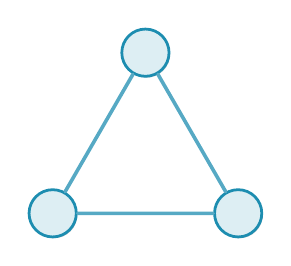
\begin{tikzpicture}[scale=1.6]
  \node[gvertex] (u1) at (90:0.85) {};
  \node[gvertex] (u2) at (210:0.85) {};
  \node[gvertex] (u3) at (330:0.85) {};
  \draw[gline] (u1)--(u2) (u2)--(u3) (u3)--(u1);
\end{tikzpicture}}\\[10pt]
{\footnotesize\color{black!60} value linear in $n$}

\column{0.06\textwidth}
\centering
\vspace{2.4cm}{\color{black!25}\large vs}

\column{0.47\textwidth}
\centering
{\pillicon{pillRed}}\ \ {\large\bfseries directed}\\[2pt]
{\scriptsize\color{black!60} an arc is an ordered pair}\\[12pt]
\adjustbox{max totalheight=0.355\textheight, max width=\linewidth}{%
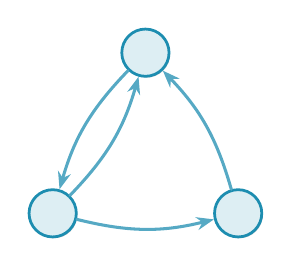
\begin{tikzpicture}[scale=1.6, >=Stealth]
  \node[gvertex] (d1) at (90:0.85) {};
  \node[gvertex] (d2) at (210:0.85) {};
  \node[gvertex] (d3) at (330:0.85) {};
  \draw[gdir] (d1) to[bend right=14] (d2);
  \draw[gdir] (d2) to[bend right=14] (d3);
  \draw[gdir] (d3) to[bend right=14] (d1);
  \draw[gdir] (d2) to[bend right=14] (d1);
\end{tikzpicture}}\\[10pt]
{\footnotesize\color{black!60} value quadratic in $n$}
\end{columns}
\vspace{10pt}
\noindent{\footnotesize\color{black!60}
One-way traffic is the toggle that changes the order of the answer: a route
from $u$ to $v$ no longer doubles as a route from $v$ to $u$, so a graph can
hold on the order of $n^2/4$ arcs under the same cap. These are the open
cases.}\par
\end{frame}

% ============================================================================
%  DIVIDER
% ============================================================================
\begin{frame}[plain]
\vfill
\hspace*{1.4cm}\begin{minipage}{0.85\textwidth}
  {\color{black!35}\large PART II}\\[8pt]
  {\color{KULblauw3b}\fontsize{28}{32}\selectfont\bfseries The program}\\[10pt]
  {\color{black!55}\large Sixteen variants, one flow computation.}
\end{minipage}
\vfill
\end{frame}

% ============================================================================
%  8.  MODELLING: THE TWO ENCODINGS
% ============================================================================
\begin{frame}{Modelling: two encodings}
\vfill
\begin{center}
\adjustbox{max totalheight=0.60\textheight}{\resizebox{0.76\textwidth}{!}{%
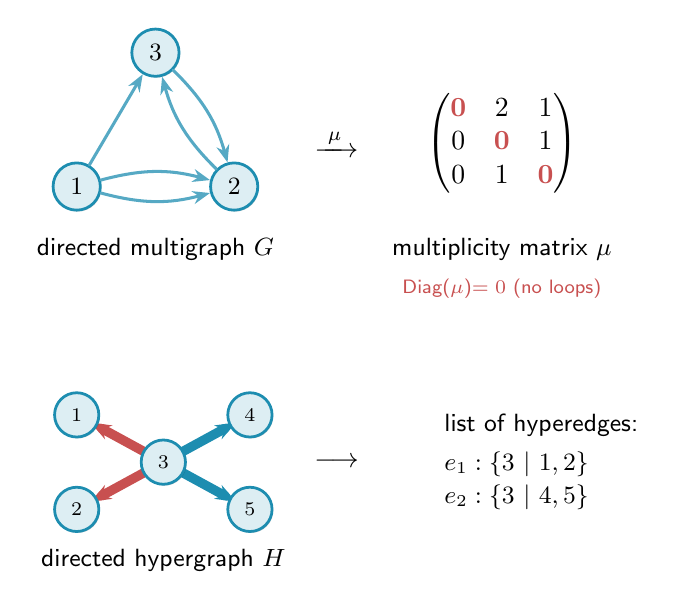
\begin{tikzpicture}[>=Stealth]
% ---- non-hypergraphs: one multiplicity matrix -----------------------------
\node[vertex] (A) at (0,   0)   {$1$};
\node[vertex] (B) at (2.0, 0)   {$2$};
\node[vertex] (C) at (1.0, 1.7) {$3$};
\draw[arc] (A) to[bend left=15]  (B);
\draw[arc] (A) to[bend right=15] (B);
\draw[arc] (B) to[bend left=15]  (C);
\draw[arc] (C) to[bend left=15]  (B);
\draw[arc] (A) -- (C);
\node[font=\small] at (1.0, -0.8) {directed multigraph $G$};
\node at (3.3, 0.55) {$\xrightarrow{\;\mu\;}$};
\node at (5.4, 0.55) {$\begin{pmatrix}
  {\color{vertexred}\mathbf 0} & 2 & 1 \\
  0 & {\color{vertexred}\mathbf 0} & 1 \\
  0 & 1 & {\color{vertexred}\mathbf 0}\end{pmatrix}$};
\node[font=\small] at (5.4, -0.8) {multiplicity matrix $\mu$};
\node[font=\scriptsize, vertexred] at (5.4, -1.3) {Diag($\mu$)$=0$ (no loops)};
% ---- hypergraphs: a list of hyperedges ------------------------------------
\begin{scope}[yshift=-3.5cm]
  \coordinate (p1) at (0.0, 0.6);
  \coordinate (p2) at (0.0,-0.6);
  \coordinate (p3) at (1.1, 0.0);
  \coordinate (p4) at (2.2, 0.6);
  \coordinate (p5) at (2.2,-0.6);
  \begin{scope}[on background layer]
    \draw[metro, metroA, -{Stealth[length=2.6mm]}, shorten >=2mm, shorten <=1.4mm] (p3) -- (p1);
    \draw[metro, metroA, -{Stealth[length=2.6mm]}, shorten >=2mm, shorten <=1.4mm] (p3) -- (p2);
    \draw[metro, metroB, -{Stealth[length=2.6mm]}, shorten >=2mm, shorten <=1.4mm] (p3) -- (p4);
    \draw[metro, metroB, -{Stealth[length=2.6mm]}, shorten >=2mm, shorten <=1.4mm] (p3) -- (p5);
  \end{scope}
  \foreach \p/\lbl in {p1/1,p2/2,p3/3,p4/4,p5/5} {\node[smallvertex] at (\p) {$\lbl$};}
  \node[font=\small] at (1.1,-1.25) {directed hypergraph $H$};
  \node at (3.3, 0.0) {$\longrightarrow$};
  \node[font=\small, align=left] at (5.9, 0.0)
    {list of hyperedges:\\[3pt] $e_1: \{3\ |\ 1,2\}$\\[1pt] $e_2:\{3\ |\ 4,5\}$};
\end{scope}
\end{tikzpicture}}}
\end{center}
\vspace{6pt}
\noindent{\footnotesize\color{black!60}
A matrix would be too large and too sparse for hyperedges, so the model splits
in two: every non-hypergraph is one multiplicity matrix, symmetric when
undirected and binary when simple, and every hypergraph is a list of vertex
sets, with the tail marked when directed.}\par
\vfill
\end{frame}

% ============================================================================
%  9.  MAX FLOW: IN AND OUT
% ============================================================================
\begin{frame}{Measuring: one max-flow computation}
\vspace{2pt}
\begin{center}
\adjustbox{max totalheight=0.56\textheight}{\resizebox{0.98\textwidth}{!}{%
\begin{tikzpicture}[>=Stealth,
   iobox/.style={rounded corners=4pt, draw=black!22, fill=black!3,
                 inner sep=9pt, align=center},
   pipe/.style={-{Stealth[length=3.4mm]}, line width=1.6pt, KULblauw1!70}]

  % ---- input --------------------------------------------------------------
  \node[iobox] (in) at (0,0) {%
    \begin{tikzpicture}[>=Stealth, scale=1.45]
      \node[smallvertex] (A) at (0,0)     {$1$};
      \node[smallvertex] (B) at (2.1,0)   {$2$};
      \node[smallvertex] (C) at (1.05,1.8){$3$};
      \draw[arc] (A) to[bend left=17]  (B);
      \draw[arc] (A) to[bend right=17] node[below, font=\scriptsize, text=black!60]{$2$} (B);
      \draw[arc] (A) -- node[left, font=\scriptsize, text=black!60]{$1$} (C);
      \draw[arc] (B) to[bend left=17]  node[right, font=\scriptsize, text=black!60, pos=0.5]{$1$} (C);
      \draw[arc] (C) to[bend left=17]  node[left,  font=\scriptsize, text=black!60, pos=0.5]{$1$} (B);
    \end{tikzpicture}};
  \node[font=\scriptsize\bfseries, text=KULblauw3b, above=2pt of in]
    {INPUT\ \ directed multigraph};
  \node[font=\scriptsize, text=black!55, below=2pt of in]
    {capacities are the multiplicities $\mu(u,v)$};

  % ---- the checker ---------------------------------------------------------
  \node[iobox, fill=KULblauw3a!12, draw=KULblauw1!45, minimum width=42mm] (box) at (6.6,0)
    {{\bfseries integer max flow}\\[3pt]
     {\scriptsize run once per ordered pair}\\[1pt]
     {\scriptsize keep the largest value}};
  \node[font=\scriptsize\bfseries, text=KULblauw3b, above=2pt of box] {THE CHECKER};

  % ---- output --------------------------------------------------------------
  \node[iobox, fill=vertexorange!8, draw=vertexorange!45] (out) at (12.4,0)
    {{\Large$\lmax_G\;=\;3$}\\[4pt]
     {\scriptsize attained at the pair $(1,2)$}};
  \node[font=\scriptsize\bfseries, text=KULblauw3b, above=2pt of out]
    {OUTPUT\ \ one number};

  \draw[pipe] (in) -- (box);
  \draw[pipe] (box) -- (out);
\end{tikzpicture}}}
\end{center}
\vspace{6pt}
\begin{center}
{\normalsize
$\lec_G(u,v)\;\overset{\text{Menger}}{=}\;$ smallest $u$--$v$ cut
$\;\overset{\text{Ford--Fulkerson}}{=}\;$ largest $u$--$v$ flow}
\end{center}
\vspace{4pt}
\noindent{\footnotesize\color{black!60}
So the connectivity question is a flow question, and the whole program has one
numerical primitive. Every other variant is transformed until it becomes this
input.}\par
\end{frame}

% ============================================================================
%  10.  TRANSFORMATIONS
% ============================================================================
\begin{frame}{Transformations: everything becomes this one input}
\vspace{4pt}
\transrow{undirected $\to$ directed}{one edge becomes two arcs}{%
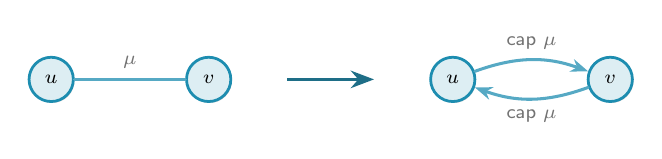
\begin{tikzpicture}[>=Stealth]
  \node[smallvertex] (u) at (0,0) {$u$};
  \node[smallvertex] (v) at (2.0,0) {$v$};
  \draw[gline] (u) -- node[above, font=\scriptsize, text=black!55]{$\mu$} (v);
  \draw[->, very thick, color=KULblauw3b] (3.0,0) -- (4.1,0);
  \node[smallvertex] (u2) at (5.1,0) {$u$};
  \node[smallvertex] (v2) at (7.1,0) {$v$};
  \draw[gdir] (u2) to[bend left=20]  node[above, font=\scriptsize, text=black!55]{cap $\mu$} (v2);
  \draw[gdir] (v2) to[bend left=20]  node[below, font=\scriptsize, text=black!55]{cap $\mu$} (u2);
\end{tikzpicture}}

\vspace{9pt}
\transrow{hypergraph $\to$ graph}{a hyperedge becomes a gate}{%
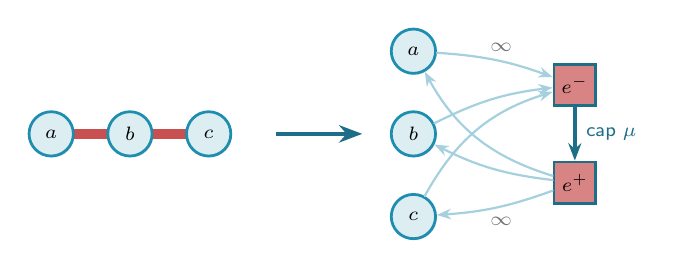
\begin{tikzpicture}[>=Stealth]
\coordinate (a) at (0.0, 0.0); \coordinate (b) at (1.0, 0.0); \coordinate (c) at (2.0, 0.0);
\begin{scope}[on background layer]\draw[metro, metroA] (a)--(b)--(c);\end{scope}
\node[smallvertex] at (a) {$a$}; \node[smallvertex] at (b) {$b$}; \node[smallvertex] at (c) {$c$};
\draw[->, very thick, color=KULblauw3b] (2.85, 0.0) -- (3.95, 0.0);
\begin{scope}[xshift=4.6cm]
\node[smallvertex] (a2) at (0.0,  1.05) {$a$};
\node[smallvertex] (b2) at (0.0,  0.00) {$b$};
\node[smallvertex] (c2) at (0.0, -1.05) {$c$};
\node[hnode, fill=metroA!70, minimum size=15pt] (em) at (2.05,  0.62) {$e^-$};
\node[hnode, fill=metroA!70, minimum size=15pt] (ep) at (2.05, -0.62) {$e^+$};
\draw[gdirfaint] (a2) to[bend left=8]  node[above, font=\scriptsize, text=black!55, pos=0.55]{$\infty$} (em);
\draw[gdirfaint] (b2) to[bend left=10] (em);
\draw[gdirfaint] (c2) to[bend left=22] (em);
\draw[gdirfaint] (ep) to[bend left=22] (a2);
\draw[gdirfaint] (ep) to[bend left=10] (b2);
\draw[gdirfaint] (ep) to[bend left=8]  node[below, font=\scriptsize, text=black!55, pos=0.45]{$\infty$} (c2);
\draw[gdir, line width=1.6pt, color=KULblauw3b] (em) -- node[right, font=\scriptsize]{cap $\mu$} (ep);
\end{scope}
\end{tikzpicture}}

\vspace{9pt}
\transrow{$\kap \to \lec$}{a vertex becomes a gate too}{%
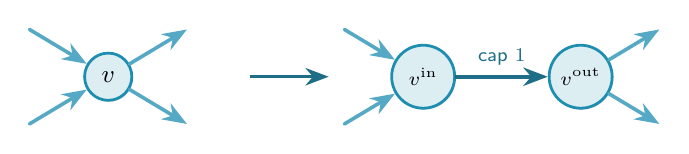
\begin{tikzpicture}[>=Stealth]
\node[vertex] (v) at (1.0, 0) {$v$};
\draw[->, edge] (0.0,  0.6) -- (v);
\draw[->, edge] (0.0, -0.6) -- (v);
\draw[->, edge] (v) -- (2.0,  0.6);
\draw[->, edge] (v) -- (2.0, -0.6);
\draw[->, very thick, color=KULblauw3b] (2.8, 0) -- (3.8, 0);
\node[smallvertex, minimum size=8mm] (vi) at (5.0, 0) {$v^{\mathrm{in}}$};
\node[smallvertex, minimum size=8mm] (vo) at (7.0, 0) {$v^{\mathrm{out}}$};
\draw[->, edge, color=KULblauw3b] (vi) -- node[above, font=\scriptsize]{cap $1$} (vo);
\draw[->, edge] (4.0,  0.6) -- (vi);
\draw[->, edge] (4.0, -0.6) -- (vi);
\draw[->, edge] (vo) -- (8.0,  0.6);
\draw[->, edge] (vo) -- (8.0, -0.6);
\end{tikzpicture}}

\vspace{9pt}
\noindent{\footnotesize\color{black!60}
A gate is the only bottleneck on the routes through it, so its capacity is
exactly what a route must spend. The three are applied in this order, and the
gates themselves are never split.}\par
\end{frame}

% ============================================================================
%  11.  EFFICIENCY
% ============================================================================
\begin{frame}{Efficiency: three ways to make the sweep finish}
\vspace{2pt}
\begin{columns}[T,onlytextwidth]

% ---- pruning --------------------------------------------------------------
\column{0.315\textwidth}
\centering
{\color{KULblauw3b}\bfseries Pruning}\\[1pt]
{\scriptsize\color{black!55} cut a branch, not a graph}\\[8pt]
\adjustbox{max totalheight=0.355\textheight, max width=\linewidth}{%
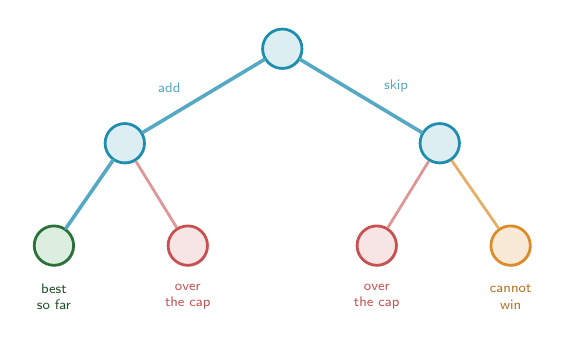
\begin{tikzpicture}[scale=1.0, >=Stealth,
   live/.style={gvertex, minimum size=5mm},
   dead/.style={gvsink, minimum size=5mm},
   bnd/.style={gvhub, minimum size=5mm},
   best/.style={gvertex, draw=vertexgreen!70!black, fill=vertexgreen!18, minimum size=5mm}]
  \node[live] (r)  at (0,0)       {};
  \node[live] (l)  at (-2.0,-1.2) {};
  \node[live] (rr) at (2.0,-1.2)  {};
  \draw[gline] (r) -- node[above left,  font=\tiny, pos=0.6]{add} (l);
  \draw[gline] (r) -- node[above right, font=\tiny, pos=0.6]{skip} (rr);
  \node[best] (l1) at (-2.9,-2.5) {};
  \node[dead] (l2) at (-1.2,-2.5) {};
  \node[dead] (r1) at (1.2,-2.5)  {};
  \node[bnd]  (r2) at (2.9,-2.5)  {};
  \draw[gline] (l)--(l1);
  \draw[line width=1pt, vertexred!60] (l)--(l2);
  \draw[line width=1pt, vertexred!60] (rr)--(r1);
  \draw[line width=1pt, vertexorange!70] (rr)--(r2);
  \node[font=\tiny, vertexgreen!50!black, align=center] at (-2.9,-3.15) {best\\so far};
  \node[font=\tiny, vertexred, align=center]    at (-1.2,-3.15) {over\\the cap};
  \node[font=\tiny, vertexred, align=center]    at (1.2,-3.15)  {over\\the cap};
  \node[font=\tiny, vertexorange!80!black, align=center] at (2.9,-3.15) {cannot\\win};
\end{tikzpicture}}\\[6pt]
{\scriptsize\color{black!60}
Adding an edge never lowers connectivity, so a partial graph already over the
cap condemns every completion.}

% ---- generating search ----------------------------------------------------
\column{0.315\textwidth}
\centering
{\color{KULblauw3b}\bfseries Generating search}\\[1pt]
{\scriptsize\color{black!55} do not check the same graph twice}\\[8pt]
\adjustbox{max totalheight=0.355\textheight, max width=\linewidth}{%
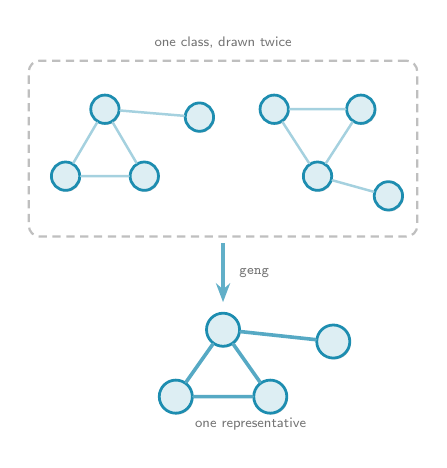
\begin{tikzpicture}[scale=1.0, >=Stealth, tiny/.style={gvertex, minimum size=3.6mm}]
  % two drawings of one and the same isomorphism class
  \begin{scope}[shift={(-1.15,0)}]
    \node[tiny](a1) at (0,0.5){}; \node[tiny](a2) at (-0.5,-0.35){};
    \node[tiny](a3) at (0.5,-0.35){}; \node[tiny](a4) at (1.2,0.4){};
    \draw[gfaint] (a1)--(a2) (a2)--(a3) (a3)--(a1) (a1)--(a4);
  \end{scope}
  \begin{scope}[shift={(1.55,0)}]
    \node[tiny](b1) at (0,-0.35){}; \node[tiny](b2) at (0.55,0.5){};
    \node[tiny](b3) at (-0.55,0.5){}; \node[tiny](b4) at (0.9,-0.6){};
    \draw[gfaint] (b1)--(b2) (b2)--(b3) (b3)--(b1) (b1)--(b4);
  \end{scope}
  \node[draw=black!25, densely dashed, rounded corners=4pt, line width=0.8pt,
        fit={(-2.0,-1.0) (2.7,1.0)}] (bag) {};
  \node[font=\tiny, text=black!55, anchor=south] at (0.35,1.15)
    {one class, drawn twice};
  \draw[-{Stealth[length=2.4mm]}, line width=1.2pt, KULblauw1!70]
    (0.35,-1.2) -- (0.35,-1.95) node[midway, right=2pt, font=\tiny, text=black!55]{\texttt{geng}};
  \begin{scope}[shift={(0.35,-2.75)}]
    \node[gvertex, minimum size=4.2mm](d1) at (0,0.45){};
    \node[gvertex, minimum size=4.2mm](d2) at (-0.6,-0.4){};
    \node[gvertex, minimum size=4.2mm](d3) at (0.6,-0.4){};
    \node[gvertex, minimum size=4.2mm](d4) at (1.4,0.3){};
    \draw[gline] (d1)--(d2) (d2)--(d3) (d3)--(d1) (d1)--(d4);
  \end{scope}
  \node[font=\tiny, text=black!55] at (0.7,-3.5) {one representative};
\end{tikzpicture}}\\[6pt]
{\scriptsize\color{black!60}
\texttt{nauty}'s \texttt{geng} lists one support per class; the program then
decorates its edges with arc multiplicities.}

% ---- the C helper ---------------------------------------------------------
\column{0.315\textwidth}
\centering
{\color{KULblauw3b}\bfseries A compiled inner loop}\\[1pt]
{\scriptsize\color{black!55} the same flow, faster}\\[8pt]
\adjustbox{max totalheight=0.355\textheight, max width=\linewidth}{%
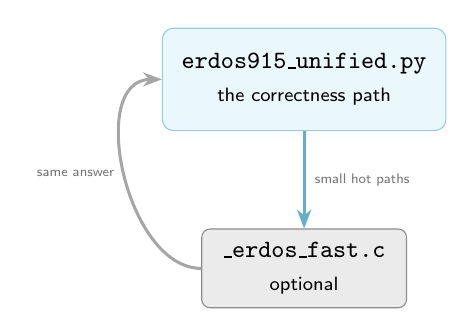
\begin{tikzpicture}[>=Stealth]
  \node[rounded corners=4pt, draw=KULblauw1!45, fill=KULblauw3a!12,
        minimum width=36mm, minimum height=13mm, align=center, font=\small]
        (py) at (0,0) {\texttt{erdos915\_unified.py}\\[1pt]{\scriptsize the correctness path}};
  \node[rounded corners=3pt, draw=black!45, fill=black!8,
        minimum width=26mm, minimum height=10mm, align=center, font=\small]
        (c) at (0,-2.4) {\texttt{\_erdos\_fast.c}\\[1pt]{\scriptsize optional}};
  \draw[-{Stealth[length=2.4mm]}, line width=1.1pt, KULblauw1!70]
    (py.south) -- node[right, font=\tiny, text=black!55]{small hot paths} (c.north);
  \draw[-{Stealth[length=2.4mm]}, line width=1.1pt, black!35]
    (c.west) to[out=180,in=180] node[left, font=\tiny, text=black!55]{same answer} (py.west);
\end{tikzpicture}}\\[6pt]
{\scriptsize\color{black!60}
Capacities too large for safe \texttt{int32} arithmetic fall back to the Python
integer path, so a speed-up cannot change an answer.}

\end{columns}
\vspace{9pt}
\noindent{\footnotesize\color{black!60}
None of the three changes what is proved. Only infeasible branches and branches
that cannot beat the incumbent are discarded, so a sweep that finishes returns
exactly what the blind walk would have returned.}\par
\end{frame}

% ============================================================================
%  12.  SOLVING vs SEARCHING
% ============================================================================
\begin{frame}{Solving versus searching}
\vspace{2pt}
\begin{center}
\adjustbox{max totalheight=0.20\textheight}{\resizebox{0.66\textwidth}{!}{%
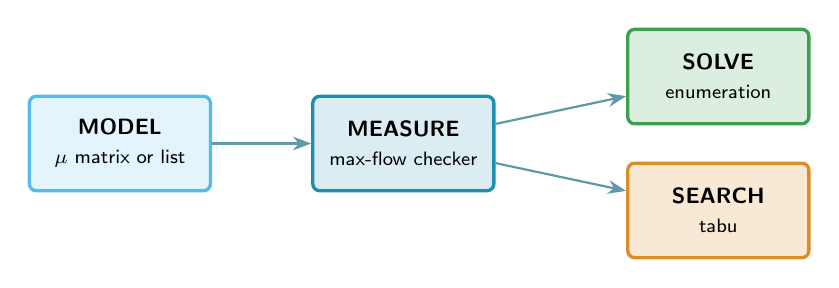
\begin{tikzpicture}[>=Stealth,
  rolenode/.style={rounded corners=2.5pt, draw, very thick, align=center,
     minimum width=23mm, minimum height=12mm, font=\sffamily\footnotesize},
  flow/.style={->, thick, KULblauw3b!70}]
  \node[rolenode, fill=roleModel!16,    draw=roleModel]    (mod) at (0,0)     {\textbf{MODEL}\\[1pt]\scriptsize $\mu$ matrix or list};
  \node[rolenode, fill=roleMeasure!16,  draw=roleMeasure]  (mea) at (3.6,0)   {\textbf{MEASURE}\\[1pt]\scriptsize max-flow checker};
  \node[rolenode, fill=roleProve!18,    draw=roleProve]    (pro) at (7.6,0.85){\textbf{SOLVE}\\[1pt]\scriptsize enumeration};
  \node[rolenode, fill=roleDiscover!20, draw=roleDiscover] (dis) at (7.6,-0.85){\textbf{SEARCH}\\[1pt]\scriptsize tabu};
  \draw[flow] (mod) -- (mea);
  \draw[flow] (mea) -- (pro);
  \draw[flow] (mea) -- (dis);
\end{tikzpicture}}}
\end{center}
\vspace{10pt}
\begin{columns}[T,onlytextwidth]
\column{0.47\textwidth}
{\large\color{vertexgreen!55!black}\bfseries Solving}\\[2pt]
{\scriptsize\color{black!55} walk the whole space}
\vspace{7pt}
\begin{itemize}\setlength{\itemsep}{4pt}\small
  \item[\color{vertexgreen!60!black}\textbullet] every graph on $n$ vertices, measured
  \item[\color{vertexgreen!60!black}\textbullet] \textbf{finishes} $\Rightarrow$ the exact value at that $n$, upper bound included
  \item[\color{vertexgreen!60!black}\textbullet] \textbf{times out} $\Rightarrow$ only the best graph seen, a lower bound
\end{itemize}

\column{0.06\textwidth}
\centering\vspace{0.9cm}{\color{black!22}\large vs}

\column{0.47\textwidth}
{\large\color{vertexorange!80!black}\bfseries Searching}\\[2pt]
{\scriptsize\color{black!55} steer through the space}
\vspace{7pt}
\begin{itemize}\setlength{\itemsep}{4pt}\small
  \item[\color{vertexorange!85!black}\textbullet] tabu search on the energy $\Phi$, from the empty graph
  \item[\color{vertexorange!85!black}\textbullet] reaches sizes the sweep cannot
  \item[\color{vertexorange!85!black}\textbullet] \textbf{always} exhibits a graph, so \textbf{always} only a lower bound
\end{itemize}
\end{columns}
\vspace{8pt}
\hspace*{0.9cm}{\color{KULblauw3a}\rule{0.82\paperwidth}{1.1pt}}
\vspace{7pt}
\begin{center}
{\normalsize\color{KULblauw3b}\bfseries
A value is settled only where a proof and a construction meet.}
\end{center}
\end{frame}

% ============================================================================
%  13.  THE SEARCH: ONE NUMBER PER GRAPH
% ============================================================================
\begin{frame}{The search: one number per graph}
\vspace{6pt}
\begin{center}
{\large
$\Phi(G)\;=\;
 \underbrace{-\,|E(G)|}_{\substack{\text{\normalsize reward}\\[1pt]
   \text{\scriptsize\color{black!55} more edges, lower energy}}}
 \;+\;
 \underbrace{\Lambda\cdot\max\bigl(0,\;c^{\max}(G)-(m-1)\bigr)}
   _{\substack{\text{\normalsize penalty}\\[1pt]
   \text{\scriptsize\color{black!55} $\Lambda$ large, so breaking the cap never pays}}}$}
\end{center}
\vspace{22pt}
\begin{center}
\adjustbox{max totalheight=0.30\textheight}{\resizebox{0.80\textwidth}{!}{%
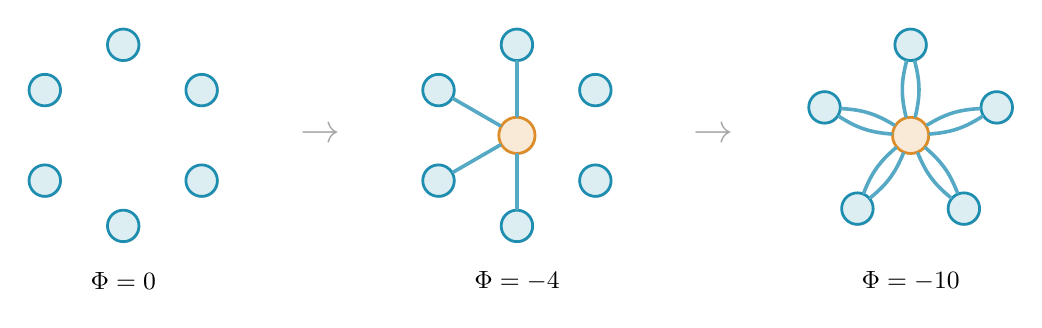
\begin{tikzpicture}[>=Stealth, tv/.style={gvertex, minimum size=4mm}]
  \begin{scope}[shift={(0,0)}]
    \foreach \ang in {90,150,210,270,330,30} {\node[tv] at (\ang:1.15) {};}
    \node[font=\small] at (0,-1.85) {$\Phi=0$};
  \end{scope}
  \node[font=\Large, text=black!35] at (2.5,0) {$\to$};
  \begin{scope}[shift={(5.0,0)}]
    \node[gvhub, minimum size=4.6mm] (h) at (0,0) {};
    \foreach \ang in {90,150,210,270} {\node[tv] (p\ang) at (\ang:1.15) {};
      \draw[gline] (h) -- (p\ang);}
    \foreach \ang in {330,30} {\node[tv] at (\ang:1.15) {};}
    \node[font=\small] at (0,-1.85) {$\Phi=-4$};
  \end{scope}
  \node[font=\Large, text=black!35] at (7.5,0) {$\to$};
  \begin{scope}[shift={(10.0,0)}]
    \node[gvhub, minimum size=4.6mm] (h2) at (0,0) {};
    \foreach \ang in {90,162,234,306,18} {\node[tv] (q\ang) at (\ang:1.15) {};
      \draw[gline] (h2) to[gcurve]  (q\ang);
      \draw[gline] (h2) to[gcurveR] (q\ang);}
    \node[font=\small] at (0,-1.85) {$\Phi=-10$};
  \end{scope}
\end{tikzpicture}}}
\end{center}
\vspace{6pt}
\noindent{\footnotesize\color{black!60}
Tabu search, started from the empty graph on $n=6$ at $m=3$, walks downhill in
$\Phi$ and forbids recently touched edges so it cannot walk straight back.
Its endpoint here, the multiplicity-$2$ star with ten edges, is the known
extremiser $L_3(6)=10$.}\par
\end{frame}

% ============================================================================
%  14.  WHAT THE SEARCH REDISCOVERS
% ============================================================================
\tikzframescaled{What the search finds on its own}{%
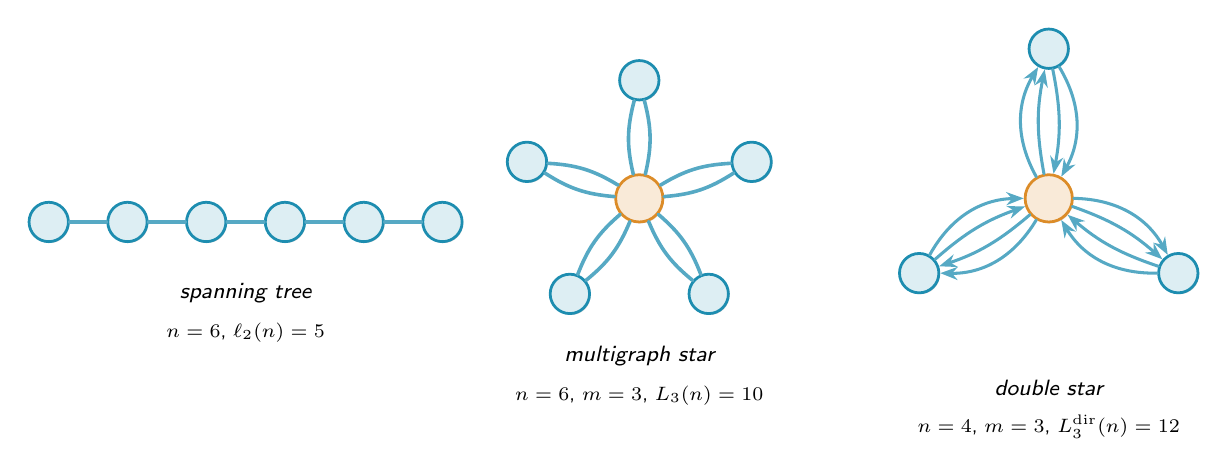
\begin{tikzpicture}[>=Stealth]
  \begin{scope}[shift={(-7.5,0)}]
    \foreach \i/\x in {1/0,2/1.0,3/2.0,4/3.0,5/4.0,6/5.0} {
      \node[gvertex, minimum size=5mm] (t\i) at (\x,0) {};
    }
    \foreach \i/\j in {1/2,2/3,3/4,4/5,5/6} {\draw[gline] (t\i) -- (t\j);}
    \node[font=\footnotesize\itshape] at (2.5,-0.9) {spanning tree};
    \node[font=\scriptsize] at (2.5,-1.4) {$n=6$, $\ell_2(n)=5$};
  \end{scope}
  \begin{scope}[shift={(0,0.3)}]
    \node[gvhub, minimum size=6mm] (h2) at (0,0) {};
    \foreach \ang in {90,162,234,306,18} {
      \node[gvertex, minimum size=5mm] (l2\ang) at (\ang:1.5) {};
      \draw[gline] (h2) to[gcurve]  (l2\ang);
      \draw[gline] (h2) to[gcurveR] (l2\ang);
    }
    \node[font=\footnotesize\itshape] at (0,-2.0) {multigraph star};
    \node[font=\scriptsize] at (0,-2.5) {$n=6$, $m=3$, $L_3(n)=10$};
  \end{scope}
  \begin{scope}[shift={(5.2,0.3)}]
    \node[gvhub, minimum size=6mm] (h3) at (0,0) {};
    \foreach \ang in {90,210,330} {
      \node[gvertex, minimum size=5mm] (l3\ang) at (\ang:1.9) {};
      \draw[gdir] (h3)     to[bend left=30]  (l3\ang);
      \draw[gdir] (h3)     to[bend left=11]  (l3\ang);
      \draw[gdir] (l3\ang) to[bend left=30]  (h3);
      \draw[gdir] (l3\ang) to[bend left=11]  (h3);
    }
    \node[font=\footnotesize\itshape] at (0,-2.4) {double star};
    \node[font=\scriptsize] at (0,-2.9) {$n=4$, $m=3$, $L_3^{\dir}(n)=12$};
  \end{scope}
\end{tikzpicture}}{%
Told only to pack in edges, the search returns the named constructions. That is
the check on the machine. It still only ever exhibits a graph, so it proposes a
lower bound and never an upper one.}{0.95}

% ============================================================================
%  15.  THE SIXTEEN VARIANTS
% ============================================================================
\begin{frame}{Status of the sixteen variants}
\vspace{-4pt}
\begin{center}
\adjustbox{max totalheight=0.62\textheight}{\resizebox{\textwidth}{!}{%
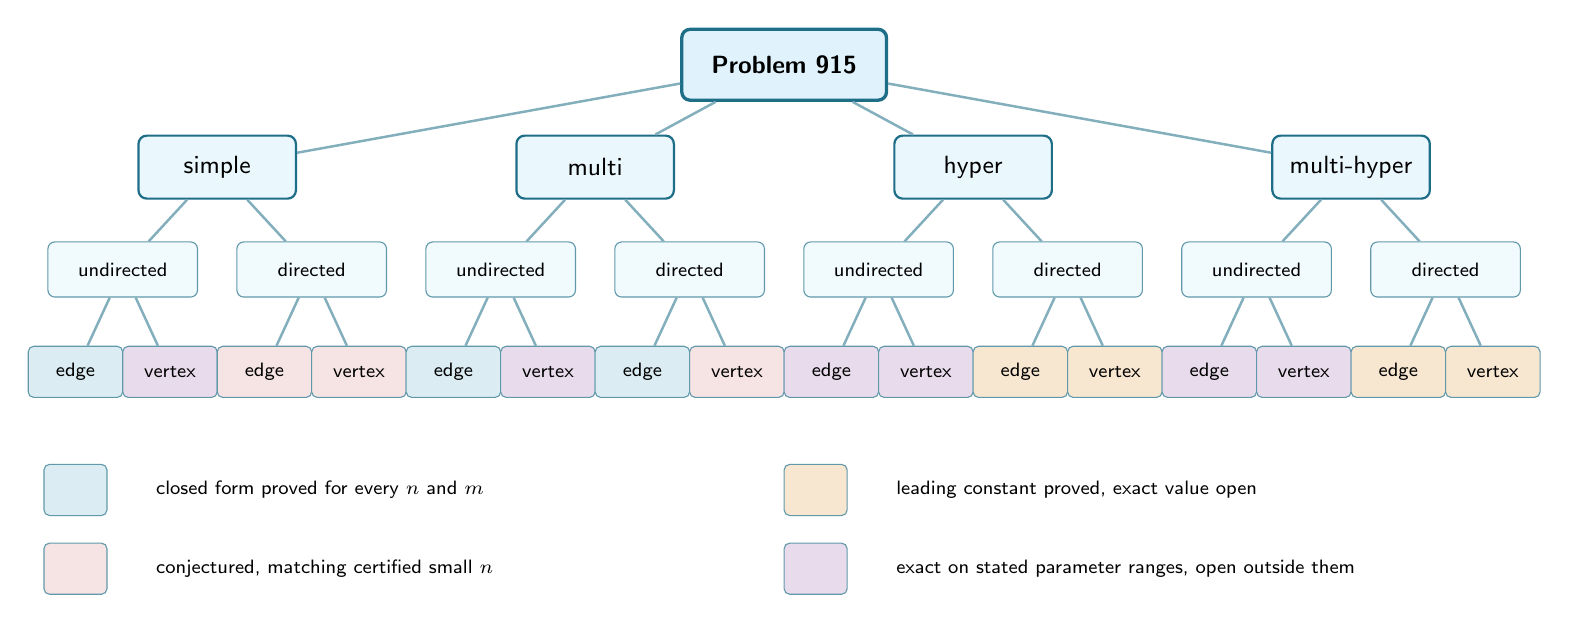
\begin{tikzpicture}
  \node[vtroot, fill=KULblauw3a!18]  (root) at (9.0,3.9) {Problem 915};
  \node[vtmodel, fill=KULblauw3a!12] (simple) at (1.8,2.6)  {simple};
  \node[vtmodel, fill=KULblauw3a!12] (multi)  at (6.6,2.6)  {multi};
  \node[vtmodel, fill=KULblauw3a!12] (hyper)  at (11.4,2.6) {hyper};
  \node[vtmodel, fill=KULblauw3a!12] (mhyper) at (16.2,2.6) {multi-hyper};
  \draw[vtedge] (root) -- (simple);
  \draw[vtedge] (root) -- (multi);
  \draw[vtedge] (root) -- (hyper);
  \draw[vtedge] (root) -- (mhyper);
  \node[vtdir, fill=KULblauw3a!8]  (d0) at (0.6,1.3)  {undirected};
  \node[vtdir, fill=KULblauw3a!8]  (d1) at (3.0,1.3)  {directed};
  \node[vtdir, fill=KULblauw3a!8]  (d2) at (5.4,1.3)  {undirected};
  \node[vtdir, fill=KULblauw3a!8]  (d3) at (7.8,1.3)  {directed};
  \node[vtdir, fill=KULblauw3a!8]  (d4) at (10.2,1.3) {undirected};
  \node[vtdir, fill=KULblauw3a!8]  (d5) at (12.6,1.3) {directed};
  \node[vtdir, fill=KULblauw3a!8]  (d6) at (15.0,1.3) {undirected};
  \node[vtdir, fill=KULblauw3a!8]  (d7) at (17.4,1.3) {directed};
  \draw[vtedge] (simple) -- (d0);
  \draw[vtedge] (simple) -- (d1);
  \draw[vtedge] (multi)  -- (d2);
  \draw[vtedge] (multi)  -- (d3);
  \draw[vtedge] (hyper)  -- (d4);
  \draw[vtedge] (hyper)  -- (d5);
  \draw[vtedge] (mhyper) -- (d6);
  \draw[vtedge] (mhyper) -- (d7);
  \node[vtleaf, fill=regimeProved!16]      (l0)  at (0,0)    {edge};
  \node[vtleaf, fill=regimePartial!20]     (l1)  at (1.2,0)  {vertex};
  \node[vtleaf, fill=regimeConjectured!16] (l2)  at (2.4,0)  {edge};
  \node[vtleaf, fill=regimeConjectured!16] (l3)  at (3.6,0)  {vertex};
  \node[vtleaf, fill=regimeProved!16]      (l4)  at (4.8,0)  {edge};
  \node[vtleaf, fill=regimePartial!20]     (l5)  at (6.0,0)  {vertex};
  \node[vtleaf, fill=regimeProved!16]      (l6)  at (7.2,0)  {edge};
  \node[vtleaf, fill=regimeConjectured!16] (l7)  at (8.4,0)  {vertex};
  \node[vtleaf, fill=regimePartial!20]     (l8)  at (9.6,0)  {edge};
  \node[vtleaf, fill=regimePartial!20]     (l9)  at (10.8,0) {vertex};
  \node[vtleaf, fill=regimeOpen!22]        (l10) at (12.0,0) {edge};
  \node[vtleaf, fill=regimeOpen!22]        (l11) at (13.2,0) {vertex};
  \node[vtleaf, fill=regimePartial!20]     (l12) at (14.4,0) {edge};
  \node[vtleaf, fill=regimePartial!20]     (l13) at (15.6,0) {vertex};
  \node[vtleaf, fill=regimeOpen!22]        (l14) at (16.8,0) {edge};
  \node[vtleaf, fill=regimeOpen!22]        (l15) at (18.0,0) {vertex};
  \draw[vtedge] (d0) -- (l0);  \draw[vtedge] (d0) -- (l1);
  \draw[vtedge] (d1) -- (l2);  \draw[vtedge] (d1) -- (l3);
  \draw[vtedge] (d2) -- (l4);  \draw[vtedge] (d2) -- (l5);
  \draw[vtedge] (d3) -- (l6);  \draw[vtedge] (d3) -- (l7);
  \draw[vtedge] (d4) -- (l8);  \draw[vtedge] (d4) -- (l9);
  \draw[vtedge] (d5) -- (l10); \draw[vtedge] (d5) -- (l11);
  \draw[vtedge] (d6) -- (l12); \draw[vtedge] (d6) -- (l13);
  \draw[vtedge] (d7) -- (l14); \draw[vtedge] (d7) -- (l15);
  \node[vtleaf, fill=regimeProved!16, minimum width=8mm]      (leg1) at (0,-1.5) {};
  \node[anchor=west, font=\scriptsize] at (0.9,-1.5) {closed form proved for every $n$ and $m$};
  \node[vtleaf, fill=regimeConjectured!16, minimum width=8mm] (leg2) at (0,-2.5) {};
  \node[anchor=west, font=\scriptsize] at (0.9,-2.5) {conjectured, matching certified small $n$};
  \node[vtleaf, fill=regimeOpen!22, minimum width=8mm]        (leg3) at (9.4,-1.5) {};
  \node[anchor=west, font=\scriptsize] at (10.3,-1.5) {leading constant proved, exact value open};
  \node[vtleaf, fill=regimePartial!20, minimum width=8mm]     (leg4) at (9.4,-2.5) {};
  \node[anchor=west, font=\scriptsize] at (10.3,-2.5) {exact on stated parameter ranges, open outside them};
\end{tikzpicture}}}
\end{center}
\vspace{2pt}
\noindent{\tiny\color{black!60}
Every leaf is one extremal function and its colour is that leaf's status. The
open and conjectural leaves sit in the directed half of the tree.}\par
\end{frame}

% ============================================================================
%  16.  WHAT IS NEW
% ============================================================================
\begin{frame}{What is new here}
\vfill
\begin{itemize}\setlength{\itemsep}{13pt}
  \item[\color{KULblauw1}\textbf{1}] \textbf{One-way multigraphs, solved for every $n$ and every $m$}\\
        {\small\color{black!60} $L_m^{\dir}(n)=(m-1)\max\bigl(2(n-1),\floorfrac{n^2}{4}\bigr)$, by deleting a sparse reachability-preserving subgraph once per unit of $m-1$ rather than a vertex at a time. The quadratic extremisers are classified for $n\ge\max(8,2m)$.}
  \item[\color{KULblauw1}\textbf{2}] \textbf{One-way simple graphs: an unconditional quadratic bound}\\
        {\small\color{black!60} $|A(D)|\le\floorfrac{n^2}{4}+4(m-1)(n-1)$, with no hypothesis on the shape of the extremiser, so the leading constant and the order of the next term are theorems. The same count re-runs under the stricter separation.}
  \item[\color{KULblauw1}\textbf{3}] \textbf{Hyperedge networks: the vertex problem at $m=2$ and $m=3$, and a directed leading term}\\
        {\small\color{black!60} $\floor{2(n-1)/(r-1)}$ is a universal $m=3$ bound from a new incidence-graph rank lemma, attained for $r\ge3$ when $2\le\binom{n-2}{r-2}$. One-way, the leading term is $(m-1)n^2/\bigl(4(r-1)\bigr)$ under both separations.}
\end{itemize}
\vfill
\end{frame}

% ============================================================================
%  17.  WHAT IS LEFT
% ============================================================================
\begin{frame}{What is left}
\vfill
\begin{itemize}\setlength{\itemsep}{12pt}
  \item[{\color{regimePartial}$\blacksquare$}] The undirected \emph{vertex} problem at $m\ge6$, open since 1974
  \item[{\color{regimeConjectured}$\blacksquare$}] The decomposition that would turn the directed conjecture into a theorem: that every extremal non-hub digraph splits as $A\cup B$ with no arc coming back
  \item[{\color{regimeConjectured}$\blacksquare$}] Whether the directed vertex value equals the arc value at $m\ge3$, which Whitney's inequality does not hand over
  \item[{\color{regimeOpen}$\blacksquare$}] The exact values behind the leading terms now settled, one-way and for hyperedges alike
\end{itemize}

\vspace{22pt}
\centering
{\color{black!55}\small The map is filled in where the arguments reached,}\\[3pt]
{\color{black!55}\small and the blanks are marked where they did not.}
\vfill
\end{frame}

% ============================================================================
%  18.  AI
% ============================================================================
\begin{frame}{AI: curse or blessing?}
\vspace{4pt}
\begin{columns}[T,onlytextwidth]
\column{0.48\textwidth}
{\large\color{vertexgreen!60!black}\bfseries Pros}
\begin{itemize}
\item \LaTeX{} typesetting
\item length \& complexity of generated text
\end{itemize}
\column{0.48\textwidth}
{\large\color{vertexred}\bfseries Cons}
\begin{itemize}
\item length \& complexity of generated text
\item control
\end{itemize}
\end{columns}
\vspace{8pt}
\hspace*{0.9cm}{\color{KULblauw3a}\rule{0.82\paperwidth}{1.1pt}}
\vfill
\begin{center}
{\Large\color{KULblauw3b}\bfseries It's a tool.}\\[8pt]
{\normalsize short leash\ \ $+$\ \ AI proofs\ \ $=$\ \ argumented conjecture\ \aimedal}
\end{center}
\vfill
\end{frame}

\end{document}
